\section{Phạm vi sáu thử nghiệm}
Để đánh giá ảnh hưởng của cách biểu diễn đặc trưng và của việc loại bỏ đặc trưng nhiễu, đề tài thiết kế sáu thử nghiệm. Tất cả thử nghiệm dùng chung một cách chia tập dữ liệu (tập Fit 19\,236 mẫu -- Validation 4\,810 mẫu -- tập kiểm tra 6\,012 mẫu), cùng một bộ thuật toán và cùng một quy trình tinh chỉnh siêu tham số; chỉ có tập đặc trưng đầu vào là thay đổi. Ngưỡng quyết định của mỗi cấu hình được chọn trên tập Validation theo F2-Score với Precision tối thiểu 0{.}6, rồi mới đánh giá một lần duy nhất trên tập kiểm tra gồm 6\,012 giao dịch, trong đó có 27 giao dịch gian lận và 5\,985 giao dịch hợp lệ.

Bên cạnh các chỉ số đã trình bày ở phần trước, mỗi bảng kết quả dưới đây báo cáo thêm hai tỷ lệ lỗi phản ánh trực tiếp rủi ro của hệ thống. Tỷ lệ bỏ sót gian lận, viết tắt FNR, là tỷ lệ giao dịch gian lận thật không bị phát hiện; tỷ lệ báo nhầm giao dịch hợp lệ, viết tắt FPR, là tỷ lệ giao dịch hợp lệ bị cảnh báo nhầm là gian lận. Sáu thử nghiệm được tóm tắt trong Bảng \ref{tab:exp_setup}.

\begin{table}[H]
\centering
\fontsize{11}{13.6}\selectfont
\renewcommand{\arraystretch}{1.2}
\setlength{\tabcolsep}{5pt}
\begin{tabularx}{\textwidth}{|>{\centering\arraybackslash}p{1.5cm}|>{\raggedright\arraybackslash}p{4.6cm}|>{\centering\arraybackslash}p{1.7cm}|X|}
\hline
\textbf{Thử nghiệm} & \textbf{Cách biểu diễn đặc trưng} & \textbf{Số đặc trưng} & \textbf{Mô hình được huấn luyện} \\
\hline
TN1 & Sáu đặc trưng gốc, chưa tạo đặc trưng mới & 6 & Random Forest, XGBoost \\
\hline
TN2 & \texttt{OneHotEncoder} cho đặc trưng phân loại & 26 & CatBoost, LightGBM, XGBoost, Random Forest \\
\hline
TN3 & \texttt{TargetEncoder} cho đặc trưng phân loại & 14 & LightGBM, Stacking, Random Forest, XGBoost, CatBoost \\
\hline
TN4 & thử nghiệm3 trừ \texttt{is\_night}, \texttt{amt\_vs\_card\_median}, \texttt{distance\_km}, \texttt{amt} & 10 & Stacking, LightGBM, XGBoost, Random Forest, CatBoost \\
\hline
TN5 & thử nghiệm3 trừ \texttt{is\_night}, \texttt{amt\_vs\_card\_median}, \texttt{distance\_km} & 11 & LightGBM, XGBoost, Random Forest, CatBoost \\
\hline
TN6 & thử nghiệm3 trừ \texttt{amt}, \texttt{amt\_vs\_card\_median}, \texttt{distance\_km} & 11 & XGBoost, LightGBM, CatBoost, Random Forest \\
\hline
\end{tabularx}
\caption{Sáu thử nghiệm đánh giá ảnh hưởng của cách mã hóa và của việc loại bỏ đặc trưng}
\label{tab:exp_setup}
\end{table}

Ba thử nghiệm đầu (TN1--TN3) giữ nguyên tập đặc trưng và chỉ thay đổi cách biểu diễn, nhằm tách ảnh hưởng của phương pháp mã hóa. Ba thử nghiệm sau (TN4--TN6) lấy thử nghiệm3 làm chuẩn và loại bỏ dần các đặc trưng mà phân tích khám phá cho thấy chứa nhiễu, nhằm kiểm tra liệu việc giảm số chiều có làm mô hình tốt hơn hay không.

\section{Kết quả từng thử nghiệm}
\subsection{Thử nghiệm 1: sáu đặc trưng gốc}
Khi chỉ dùng sáu đặc trưng gốc mà không tạo thêm đặc trưng, hiệu quả của các mô hình giảm mạnh. Random Forest đạt PR-AUC 0{.}5016 và F1-Score 0{.}5319, trong khi XGBoost thấp hơn với PR-AUC 0{.}4141. Nguyên nhân là các đặc trưng thô chưa diễn đạt được mối quan hệ phi tuyến giữa số tiền giao dịch và hành vi của chủ thẻ --- ví dụ số tiền so với mức trung bình của chính thẻ đó --- là những tín hiệu mạnh nhất trong dữ liệu. Đây là cơ sở để đề tài bổ sung nhóm đặc trưng kỹ thuật ở phần trước.

\begin{table}[H]
\centering
\fontsize{11}{13.6}\selectfont
\renewcommand{\arraystretch}{1.2}
\setlength{\tabcolsep}{4pt}
\begin{tabularx}{\textwidth}{|>{\raggedright\arraybackslash}X|>{\centering\arraybackslash}p{1.35cm}|>{\centering\arraybackslash}p{1.58cm}|>{\centering\arraybackslash}p{1.22cm}|>{\centering\arraybackslash}p{1.15cm}|>{\centering\arraybackslash}p{1.15cm}|>{\centering\arraybackslash}p{1.25cm}|>{\centering\arraybackslash}p{1.25cm}|>{\centering\arraybackslash}p{1.15cm}|>{\centering\arraybackslash}p{1.2cm}|}
\hline
\textbf{Mô hình} & \textbf{Ngưỡng} & \textbf{Precision} & \textbf{Recall} & \textbf{F1} & \textbf{F2} & \textbf{ROC-AUC} & \textbf{PR-AUC} & \textbf{FNR} & \textbf{FPR} \\
\hline
Random Forest & 0{.}1464 & 0{.}5682 & 0{.}5000 & 0{.}5319 & 0{.}5123 & 0{.}9261 & 0{.}5016 & 0{.}5000 & 0{.}0043 \\
\hline
XGBoost & 0{.}0422 & 0{.}3506 & 0{.}5400 & 0{.}4252 & 0{.}4874 & 0{.}9567 & 0{.}4141 & 0{.}4600 & 0{.}0112 \\
\hline
\end{tabularx}
\caption{Kết quả thử nghiệm1 trên tập kiểm tra với sáu đặc trưng gốc}
\label{tab:exp1}
\end{table}

\subsection{Thử nghiệm 2: mã hóa One-Hot}
Mã hóa \texttt{OneHotEncoder} làm số đặc trưng tăng lên 26 và hiệu quả tăng vượt bậc so với thử nghiệm1. Tuy nhiên đây chưa phải cấu hình tốt nhất: LightGBM đạt PR-AUC 0{.}8092 với F2-Score 0{.}7554, trong khi CatBoost đạt F2-Score cao hơn là 0{.}7801 nhờ Recall 0{.}8148, đổi lại Precision chỉ 0{.}6667. Điểm đáng chú ý là thời gian tinh chỉnh siêu tham số của LightGBM trong cấu hình này lên tới 1\,143{.}26 giây, cao hơn gấp đôi so với các thử nghiệm sau, do không gian mã hóa rời rạc làm tìm kiếm chậm hơn.

\begin{table}[H]
\centering
\fontsize{11}{13.6}\selectfont
\renewcommand{\arraystretch}{1.2}
\setlength{\tabcolsep}{4pt}
\begin{tabularx}{\textwidth}{|>{\raggedright\arraybackslash}X|>{\centering\arraybackslash}p{1.35cm}|>{\centering\arraybackslash}p{1.58cm}|>{\centering\arraybackslash}p{1.22cm}|>{\centering\arraybackslash}p{1.15cm}|>{\centering\arraybackslash}p{1.15cm}|>{\centering\arraybackslash}p{1.25cm}|>{\centering\arraybackslash}p{1.25cm}|>{\centering\arraybackslash}p{1.15cm}|>{\centering\arraybackslash}p{1.2cm}|}
\hline
\textbf{Mô hình} & \textbf{Ngưỡng} & \textbf{Precision} & \textbf{Recall} & \textbf{F1} & \textbf{F2} & \textbf{ROC-AUC} & \textbf{PR-AUC} & \textbf{FNR} & \textbf{FPR} \\
\hline
CatBoost & 0{.}6186 & 0{.}6667 & 0{.}8148 & 0{.}7333 & 0{.}7801 & 0{.}9673 & 0{.}7821 & 0{.}1852 & 0{.}0018 \\
\hline
LightGBM & 0{.}0553 & 0{.}6774 & 0{.}7778 & 0{.}7241 & 0{.}7554 & 0{.}9756 & 0{.}8092 & 0{.}2222 & 0{.}0017 \\
\hline
XGBoost & 0{.}2858 & 0{.}7143 & 0{.}7407 & 0{.}7273 & 0{.}7353 & 0{.}9721 & 0{.}7693 & 0{.}2593 & 0{.}0013 \\
\hline
Random Forest & 0{.}2100 & 0{.}7600 & 0{.}7037 & 0{.}7308 & 0{.}7143 & 0{.}9727 & 0{.}7765 & 0{.}2963 & 0{.}0010 \\
\hline
\end{tabularx}
\caption{Kết quả thử nghiệm2 trên tập kiểm tra với mã hóa \texttt{OneHotEncoder} (26 đặc trưng)}
\label{tab:exp2}
\end{table}

\subsection{Thử nghiệm 3: mã hóa Target Encoder}
Thay \texttt{OneHotEncoder} bằng \texttt{TargetEncoder} thu gọn tập đặc trưng còn 14 chiều và cho kết quả cân bằng nhất trong sáu thử nghiệm. LightGBM với \texttt{scale\_pos\_weight} đạt PR-AUC 0{.}8197, F1-Score 0{.}8163 và F2-Score 0{.}7692 --- đều là giá trị cao nhất --- với Precision 0{.}9091, Recall 0{.}7407, FPR chỉ 0{.}0003 và thời gian dự đoán 0{.}0361 giây. Stacking chỉ đứng thứ hai về PR-AUC (0{.}7820): mô hình này bắt được 21 trong 27 vụ gian lận, nhiều hơn LightGBM đúng 1 vụ, nhưng đổi lại phải báo nhầm 9 giao dịch hợp lệ so với chỉ 2 giao dịch, nên xét cả hai loại rủi ro thì Stacking không tốt bằng LightGBM.

\begin{table}[H]
\centering
\fontsize{11}{13.6}\selectfont
\renewcommand{\arraystretch}{1.2}
\setlength{\tabcolsep}{4pt}
\begin{tabularx}{\textwidth}{|>{\raggedright\arraybackslash}X|>{\centering\arraybackslash}p{1.35cm}|>{\centering\arraybackslash}p{1.58cm}|>{\centering\arraybackslash}p{1.22cm}|>{\centering\arraybackslash}p{1.15cm}|>{\centering\arraybackslash}p{1.15cm}|>{\centering\arraybackslash}p{1.25cm}|>{\centering\arraybackslash}p{1.25cm}|>{\centering\arraybackslash}p{1.15cm}|>{\centering\arraybackslash}p{1.2cm}|}
\hline
\textbf{Mô hình} & \textbf{Ngưỡng} & \textbf{Precision} & \textbf{Recall} & \textbf{F1} & \textbf{F2} & \textbf{ROC-AUC} & \textbf{PR-AUC} & \textbf{FNR} & \textbf{FPR} \\
\hline
LightGBM & 0{.}0634 & 0{.}9091 & 0{.}7407 & 0{.}8163 & 0{.}7692 & 0{.}9828 & 0{.}8197 & 0{.}2593 & 0{.}0003 \\
\hline
Stacking & 0{.}9827 & 0{.}7000 & 0{.}7778 & 0{.}7368 & 0{.}7609 & 0{.}9598 & 0{.}7820 & 0{.}2222 & 0{.}0015 \\
\hline
Random Forest & 0{.}2498 & 0{.}6897 & 0{.}7407 & 0{.}7143 & 0{.}7299 & 0{.}9516 & 0{.}7475 & 0{.}2593 & 0{.}0015 \\
\hline
XGBoost & 0{.}2545 & 0{.}5882 & 0{.}7407 & 0{.}6557 & 0{.}7042 & 0{.}9758 & 0{.}7398 & 0{.}2593 & 0{.}0023 \\
\hline
CatBoost & 0{.}8407 & 0{.}3922 & 0{.}7407 & 0{.}5128 & 0{.}6289 & 0{.}9711 & 0{.}6895 & 0{.}2593 & 0{.}0052 \\
\hline
\end{tabularx}
\caption{Kết quả thử nghiệm3 trên tập kiểm tra với mã hóa \texttt{TargetEncoder} (14 đặc trưng)}
\label{tab:exp3}
\end{table}

\subsection{Thử nghiệm 4: loại bỏ bốn đặc trưng}
Thử nghiệm 4 loại bỏ bốn đặc trưng gồm \texttt{is\_night}, \texttt{amt\_vs\_card\_median}, \texttt{distance\_km} và \texttt{amt}, còn 10 đặc trưng. LightGBM đạt PR-AUC 0{.}8231, cao nhất trong toàn bộ sáu thử nghiệm, và F1-Score 0{.}8000 gần bằng thử nghiệm 3. Tuy nhiên F2-Score giảm xuống 0{.}7634, Precision giảm còn 0{.}8696, FPR tăng gấp rưỡi lên 0{.}0005, thời gian dự đoán tăng lên 0{.}1048 giây và thời gian tinh chỉnh tăng vọt lên 2\,235{.}59 giây. Việc loại bỏ \texttt{amt} làm mô hình mất tín hiệu số tiền tuyệt đối, vốn là đặc trưng có ảnh hưởng lớn nhất theo phân tích mức độ ảnh hưởng của các đặc trưng trình bày tại Hình \ref{fig:perm_imp}.

\begin{table}[H]
\centering
\fontsize{11}{13.6}\selectfont
\renewcommand{\arraystretch}{1.2}
\setlength{\tabcolsep}{4pt}
\begin{tabularx}{\textwidth}{|>{\raggedright\arraybackslash}X|>{\centering\arraybackslash}p{1.35cm}|>{\centering\arraybackslash}p{1.58cm}|>{\centering\arraybackslash}p{1.22cm}|>{\centering\arraybackslash}p{1.15cm}|>{\centering\arraybackslash}p{1.15cm}|>{\centering\arraybackslash}p{1.25cm}|>{\centering\arraybackslash}p{1.25cm}|>{\centering\arraybackslash}p{1.15cm}|>{\centering\arraybackslash}p{1.2cm}|}
\hline
\textbf{Mô hình} & \textbf{Ngưỡng} & \textbf{Precision} & \textbf{Recall} & \textbf{F1} & \textbf{F2} & \textbf{ROC-AUC} & \textbf{PR-AUC} & \textbf{FNR} & \textbf{FPR} \\
\hline
Stacking & 0{.}9910 & 0{.}7500 & 0{.}7778 & 0{.}7636 & 0{.}7721 & 0{.}9705 & 0{.}7819 & 0{.}2222 & 0{.}0012 \\
\hline
LightGBM & 0{.}0480 & 0{.}8696 & 0{.}7407 & 0{.}8000 & 0{.}7634 & 0{.}9826 & 0{.}8231 & 0{.}2593 & 0{.}0005 \\
\hline
XGBoost & 0{.}5840 & 0{.}9048 & 0{.}7037 & 0{.}7917 & 0{.}7364 & 0{.}9808 & 0{.}7338 & 0{.}2963 & 0{.}0003 \\
\hline
Random Forest & 0{.}1387 & 0{.}5882 & 0{.}7407 & 0{.}6557 & 0{.}7042 & 0{.}9673 & 0{.}7416 & 0{.}2593 & 0{.}0023 \\
\hline
CatBoost & 0{.}8407 & 0{.}3922 & 0{.}7407 & 0{.}5128 & 0{.}6289 & 0{.}9711 & 0{.}6895 & 0{.}2593 & 0{.}0052 \\
\hline
\end{tabularx}
\caption{Kết quả thử nghiệm4 trên tập kiểm tra sau khi loại bỏ bốn đặc trưng (10 đặc trưng)}
\label{tab:exp4}
\end{table}

\subsection{Thử nghiệm 5: loại bỏ \texttt{is\_night}, \texttt{amt\_vs\_card\_median}, \texttt{distance\_km}}
Thử nghiệm 5 giữ lại \texttt{amt} nhưng loại bỏ \texttt{is\_night}, \texttt{amt\_vs\_card\_median} và \texttt{distance\_km}, còn 11 đặc trưng. LightGBM đạt PR-AUC 0{.}8205, gần bằng thử nghiệm 3, nhưng Recall giảm mạnh xuống 0{.}6667 nên F1-Score (0{.}7660) và F2-Score (0{.}7031) đều thấp hơn đáng kể, kéo theo FNR tăng lên 0{.}3333 tức bỏ sót 9 trong 27 giao dịch gian lận. Trong bốn thử nghiệm còn lại, XGBoost và CatBoost đều có PR-AUC dưới 0{.}76 và thấp hơn đáng kể so với LightGBM.

\begin{table}[H]
\centering
\fontsize{11}{13.6}\selectfont
\renewcommand{\arraystretch}{1.2}
\setlength{\tabcolsep}{4pt}
\begin{tabularx}{\textwidth}{|>{\raggedright\arraybackslash}X|>{\centering\arraybackslash}p{1.35cm}|>{\centering\arraybackslash}p{1.58cm}|>{\centering\arraybackslash}p{1.22cm}|>{\centering\arraybackslash}p{1.15cm}|>{\centering\arraybackslash}p{1.15cm}|>{\centering\arraybackslash}p{1.25cm}|>{\centering\arraybackslash}p{1.25cm}|>{\centering\arraybackslash}p{1.15cm}|>{\centering\arraybackslash}p{1.2cm}|}
\hline
\textbf{Mô hình} & \textbf{Ngưỡng} & \textbf{Precision} & \textbf{Recall} & \textbf{F1} & \textbf{F2} & \textbf{ROC-AUC} & \textbf{PR-AUC} & \textbf{FNR} & \textbf{FPR} \\
\hline
LightGBM & 0{.}1840 & 0{.}9000 & 0{.}6667 & 0{.}7660 & 0{.}7031 & 0{.}9845 & 0{.}8205 & 0{.}3333 & 0{.}0003 \\
\hline
XGBoost & 0{.}2234 & 0{.}4884 & 0{.}7778 & 0{.}6000 & 0{.}6954 & 0{.}9721 & 0{.}7584 & 0{.}2222 & 0{.}0037 \\
\hline
Random Forest & 0{.}1266 & 0{.}5405 & 0{.}7407 & 0{.}6250 & 0{.}6897 & 0{.}9478 & 0{.}7465 & 0{.}2593 & 0{.}0028 \\
\hline
CatBoost & 0{.}4779 & 0{.}6333 & 0{.}7037 & 0{.}6667 & 0{.}6884 & 0{.}9754 & 0{.}7816 & 0{.}2963 & 0{.}0018 \\
\hline
\end{tabularx}
\caption{Kết quả thử nghiệm5 trên tập kiểm tra sau khi loại bỏ ba đặc trưng (11 đặc trưng)}
\label{tab:exp5}
\end{table}

\subsection{Thử nghiệm 6: loại bỏ \texttt{amt}, \texttt{amt\_vs\_card\_median}, \texttt{distance\_km}}
Thử nghiệm 6 cũng còn 11 đặc trưng nhưng giữ lại \texttt{is\_night} thay cho \texttt{amt}. LightGBM đạt PR-AUC 0{.}8068, thấp hơn thử nghiệm 3 và là cấu hình LightGBM yếu nhất trong năm thử nghiệm; F2-Score 0{.}7364 và FNR 0{.}2963 đều kém hơn. XGBoost trong thử nghiệm 6 đạt F1 và F2 bằng nhau là 0{.}7407 do ngưỡng 0{.}2600 đặt trùng vị trí phân loại, cho thấy hiệu quả của XGBoost phụ thuộc mạnh vào tập đặc trưng hơn LightGBM.

\begin{table}[H]
\centering
\fontsize{11}{13.6}\selectfont
\renewcommand{\arraystretch}{1.2}
\setlength{\tabcolsep}{4pt}
\begin{tabularx}{\textwidth}{|>{\raggedright\arraybackslash}X|>{\centering\arraybackslash}p{1.35cm}|>{\centering\arraybackslash}p{1.58cm}|>{\centering\arraybackslash}p{1.22cm}|>{\centering\arraybackslash}p{1.15cm}|>{\centering\arraybackslash}p{1.15cm}|>{\centering\arraybackslash}p{1.25cm}|>{\centering\arraybackslash}p{1.25cm}|>{\centering\arraybackslash}p{1.15cm}|>{\centering\arraybackslash}p{1.2cm}|}
\hline
\textbf{Mô hình} & \textbf{Ngưỡng} & \textbf{Precision} & \textbf{Recall} & \textbf{F1} & \textbf{F2} & \textbf{ROC-AUC} & \textbf{PR-AUC} & \textbf{FNR} & \textbf{FPR} \\
\hline
XGBoost & 0{.}2600 & 0{.}7407 & 0{.}7407 & 0{.}7407 & 0{.}7407 & 0{.}9628 & 0{.}7480 & 0{.}2593 & 0{.}0012 \\
\hline
LightGBM & 0{.}2666 & 0{.}9048 & 0{.}7037 & 0{.}7917 & 0{.}7364 & 0{.}9808 & 0{.}8068 & 0{.}2963 & 0{.}0003 \\
\hline
CatBoost & 0{.}9023 & 0{.}8571 & 0{.}6667 & 0{.}7500 & 0{.}6977 & 0{.}9754 & 0{.}7579 & 0{.}3333 & 0{.}0005 \\
\hline
Random Forest & 0{.}1321 & 0{.}5405 & 0{.}7407 & 0{.}6250 & 0{.}6897 & 0{.}9461 & 0{.}7297 & 0{.}2593 & 0{.}0028 \\
\hline
\end{tabularx}
\caption{Kết quả thử nghiệm6 trên tập kiểm tra sau khi loại bỏ ba đặc trưng (11 đặc trưng)}
\label{tab:exp6}
\end{table}

\section{Giải thích ảnh hưởng của các đặc trưng}
Để giải thích vì sao các thử nghiệm loại bỏ đặc trưng lại cho kết quả như vậy, đề tài đo mức độ ảnh hưởng của từng đặc trưng theo phương pháp hoán đổi ngẫu nhiên, thực hiện bằng hàm \texttt{permutation\_importance} của thư viện \texttt{scikit-learn} \cite{scikitlearnpermutation}. Cụ thể, mỗi đặc trưng được hoán đổi ngẫu nhiên 10 lần và đo mức giảm PR-AUC, lấy trung bình trên 10 lần lặp. Phương pháp này đáng tin cậy hơn chỉ số độ quan trọng sẵn có của mô hình cây vì đo trực tiếp ảnh hưởng thực tế lên chất lượng dự đoán, thay vì chỉ đo mức độ chia nút. Hình \ref{fig:perm_imp} trình bày kết quả cho mô hình LightGBM tại cấu hình tốt nhất của thử nghiệm 3.

\begin{figure}[H]
    \centering
    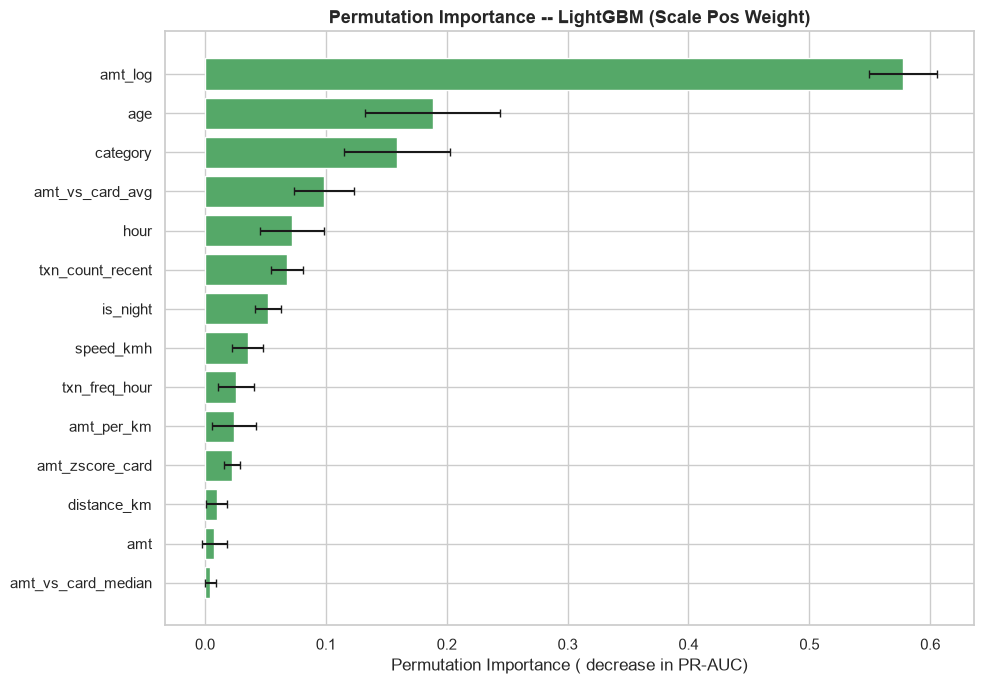
\includegraphics[width=0.9\linewidth]{figures/fig_permutation_importance_lightgbm.png}
    \caption{Mức độ ảnh hưởng của 14 đặc trưng theo phương pháp hoán đổi ngẫu nhiên, đo trên tập Validation}
    \label{fig:perm_imp}
\end{figure}

Hình \ref{fig:perm_imp} cho thấy \texttt{amt\_log} áp đảo với mức ảnh hưởng 0{.}5778, lớn hơn tổng của bốn đặc trưng đứng kế tiếp và gấp 3{.}1 lần \texttt{age} (0{.}1883); tiếp theo là \texttt{category} (0{.}1591), \texttt{amt\_vs\_card\_avg} (0{.}0982) và \texttt{hour} (0{.}0716). Ở cuối bảng là \texttt{amt\_vs\_card\_median} (0{.}0043), \texttt{amt} (0{.}0077) và \texttt{distance\_km} (0{.}0095), tức gần như không đóng góp. Kết quả này giải thích trực tiếp cho toàn bộ sáu thử nghiệm:

\begin{itemize}
    \item Vì \texttt{amt\_log} là biến dẫn xuất từ \texttt{amt}, nên khi thử nghiệm 4 loại bỏ \texttt{amt} thì đặc trưng mạnh nhất cũng biến mất, giải thích việc F2-Score và Precision của thử nghiệm 4 đều thấp hơn thử nghiệm 3.
    \item Hai đặc trưng \texttt{distance\_km} và \texttt{amt\_vs\_card\_median} có ảnh hưởng gần bằng không, nên việc loại bỏ chúng ở thử nghiệm 5 và thử nghiệm 6 không mang lại lợi ích rõ ràng --- đồng thời cho thấy chúng chỉ gây nhiễu nhẹ chứ không phải nguồn nhiễu nghiêm trọng.
    \item \texttt{is\_night} có ảnh hưởng 0{.}0521, thuộc nhóm giữa và lớn hơn rõ rệt ba đặc trưng gần như vô dụng kể trên, nên thử nghiệm 5 loại bỏ nó đã làm Recall giảm từ 0{.}7407 xuống 0{.}6667.
    \item Ba đặc trưng \texttt{is\_night}, \texttt{amt\_vs\_card\_median} và \texttt{distance\_km} mà ba thử nghiệm cuối loại bỏ có tổng ảnh hưởng chỉ khoảng 0{.}066, thấp hơn nhiều so với \texttt{amt\_log}; đây là lý do kết luận rằng việc loại bỏ đặc trưng không làm mô hình tốt hơn là có cơ sở định lượng chứ không chỉ là quan sát thực nghiệm.
\end{itemize}

\section{Tổng hợp và so sánh sáu thử nghiệm}
Bảng \ref{tab:exp_summary} và Hình \ref{fig:exp_compare} tổng hợp cấu hình tốt nhất của từng thử nghiệm. Ba kết luận nổi bật:

\begin{itemize}
    \item Kỹ thuật tạo đặc trưng quan trọng hơn phương pháp mã hóa. So sánh thử nghiệm 1 với thử nghiệm 3 cho thấy PR-AUC tăng từ 0{.}5016 lên 0{.}8197, tức tăng 63\%, chỉ nhờ bổ sung nhóm đặc trưng kỹ thuật. Trong khi đó, thay \texttt{OneHotEncoder} bằng \texttt{TargetEncoder} (thử nghiệm 2 $\to$ thử nghiệm 3) chỉ cải thiện PR-AUC từ 0{.}8092 lên 0{.}8197 nhưng lại giảm số chiều từ 26 xuống 14, giảm thời gian tinh chỉnh từ 1\,143{.}26 giây xuống 231{.}85 giây và tăng Precision từ 0{.}6774 lên 0{.}9091.
    \item Loại bỏ đặc trưng không làm mô hình tốt hơn. Cả ba thử nghiệm thử nghiệm 4--thử nghiệm 6 đều có PR-AUC của LightGBM cao hơn thử nghiệm 3 một chút (0{.}8231; 0{.}8205; 0{.}8068) nhưng đều tệ hơn ở F1-Score hoặc F2-Score, đồng thời tốn thời gian dự đoán và tinh chỉnh nhiều hơn. Chênh lệch PR-AUC giữa thử nghiệm3 và thử nghiệm4 chỉ là 0{.}0034, nhỏ hơn nhiều so với sai số do chỉ có 27 giao dịch gian lận trong tập kiểm tra: đổi số dự đoán đúng của một điểm Recall là 1/27 $\approx$ 0{.}037. Vì vậy, việc loại bỏ đặc trưng không mang lại lợi ích có ý nghĩa, và tập 14 đặc trưng của thử nghiệm3 được giữ lại.
    \item LightGBM là thuật toán bền vững nhất. Trong năm thử nghiệm có LightGBM, mô hình này dẫn đầu về PR-AUC ở cả năm thử nghiệm, đồng thời luôn giữ FPR ở mức 0{.}0003--0{.}0017, thấp hơn hẳn CatBoost (tới 0{.}0052) và XGBoost (tới 0{.}0037). Ngược lại, hiệu quả của XGBoost, CatBoost và Random Forest biến động mạnh theo tập đặc trưng: CatBoost rơi từ PR-AUC 0{.}7821 ở thử nghiệm2 xuống 0{.}6895 ở thử nghiệm3 và thử nghiệm4; XGBoost giảm từ 0{.}7693 xuống 0{.}7398.
\end{itemize}

\begin{table}[H]
\centering
\fontsize{10}{12.5}\selectfont
\renewcommand{\arraystretch}{1.2}
\setlength{\tabcolsep}{4pt}
\begin{adjustbox}{max width=\textwidth}
\begin{tabular}{|>{\centering\arraybackslash}p{1.25cm}|>{\raggedright\arraybackslash}p{3.4cm}|>{\centering\arraybackslash}p{1.2cm}|>{\centering\arraybackslash}p{1.58cm}|>{\centering\arraybackslash}p{1.22cm}|>{\centering\arraybackslash}p{1.1cm}|>{\centering\arraybackslash}p{1.1cm}|>{\centering\arraybackslash}p{1.35cm}|>{\centering\arraybackslash}p{1.45cm}|}
\hline
\textbf{TN} & \textbf{Cấu hình tốt nhất} & \textbf{Số đặc trưng} & \textbf{Precision} & \textbf{Recall} & \textbf{F1} & \textbf{F2} & \textbf{PR-AUC} & \textbf{Thời gian (s)} \\
\hline
TN1 & Random Forest & 6 & 0{.}5682 & 0{.}5000 & 0{.}5319 & 0{.}5123 & 0{.}5016 & 1{.}8849 \\
\hline
TN2 & LightGBM & 26 & 0{.}6774 & 0{.}7778 & 0{.}7241 & 0{.}7554 & 0{.}8092 & 0{.}1349 \\
\hline
TN3 & LightGBM & 14 & 0{.}9091 & 0{.}7407 & 0{.}8163 & 0{.}7692 & 0{.}8197 & 0{.}0361 \\
\hline
TN4 & LightGBM & 10 & 0{.}8696 & 0{.}7407 & 0{.}8000 & 0{.}7634 & 0{.}8231 & 0{.}1048 \\
\hline
TN5 & LightGBM & 11 & 0{.}9000 & 0{.}6667 & 0{.}7660 & 0{.}7031 & 0{.}8205 & 0{.}0941 \\
\hline
TN6 & LightGBM & 11 & 0{.}9048 & 0{.}7037 & 0{.}7917 & 0{.}7364 & 0{.}8068 & 0{.}0499 \\
\hline
\end{tabular}
\end{adjustbox}
\caption{Cấu hình tốt nhất của từng thử nghiệm trên tập kiểm tra. Với thử nghiệm1, cột thời gian ghi thời gian huấn luyện cuối cùng thay vì thời gian dự đoán, do đó không so sánh trực tiếp với năm thử nghiệm còn lại.}
\label{tab:exp_summary}
\end{table}

\begin{figure}[H]
    \centering
    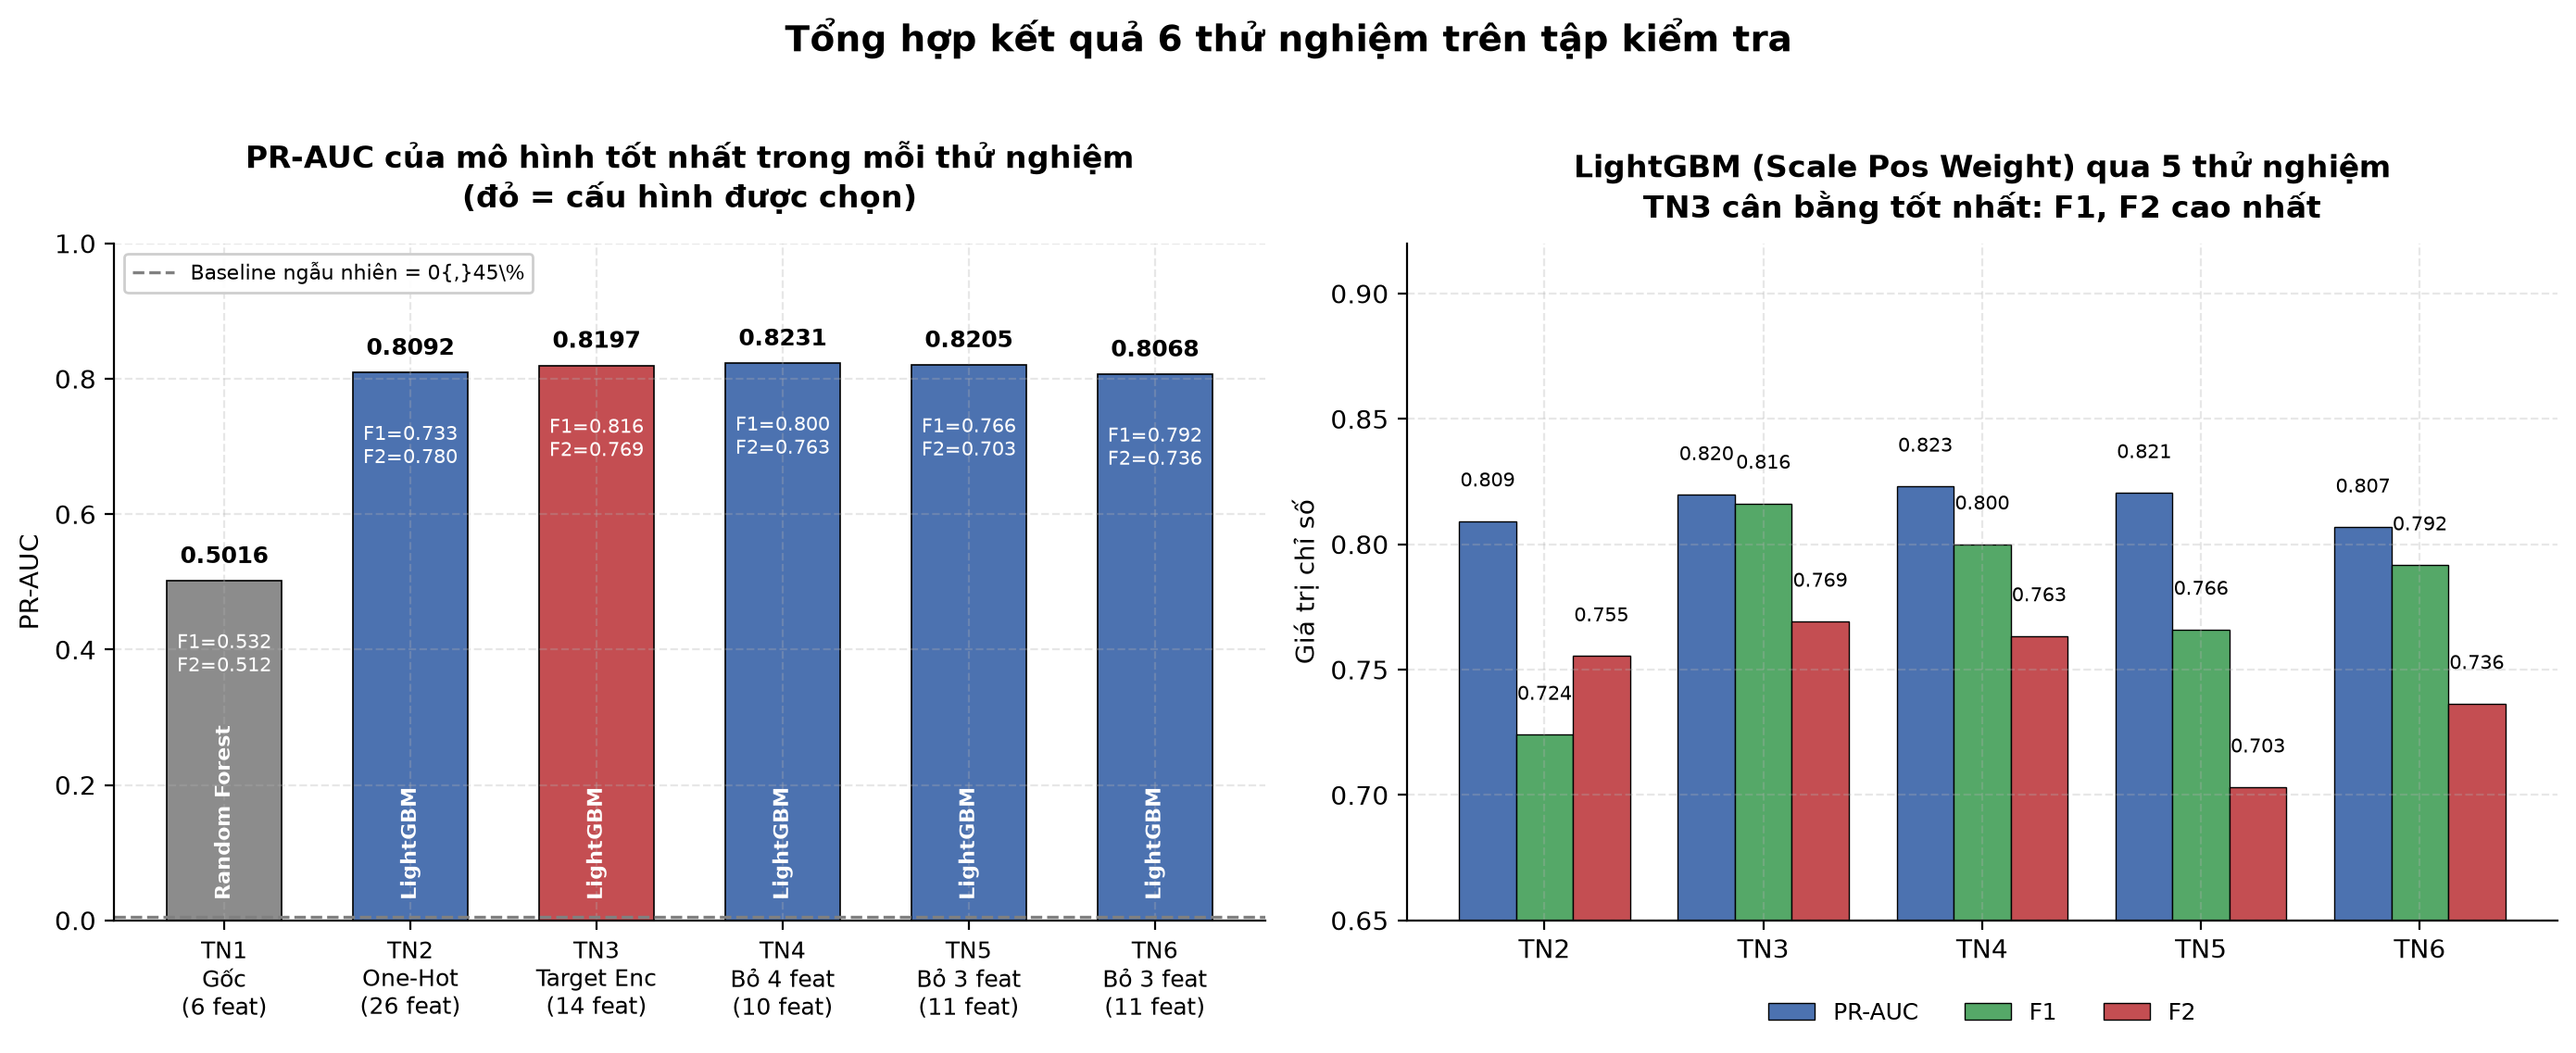
\includegraphics[width=\linewidth]{figures/fig_experiment_compare.png}
    \caption{So sánh PR-AUC của cấu hình tốt nhất trong sáu thử nghiệm (trái) và hiệu quả của LightGBM qua năm thử nghiệm (phải)}
    \label{fig:exp_compare}
\end{figure}

\section{Ma trận nhầm lẫn và đường Precision--Recall}
\begin{figure}[H]
    \centering
    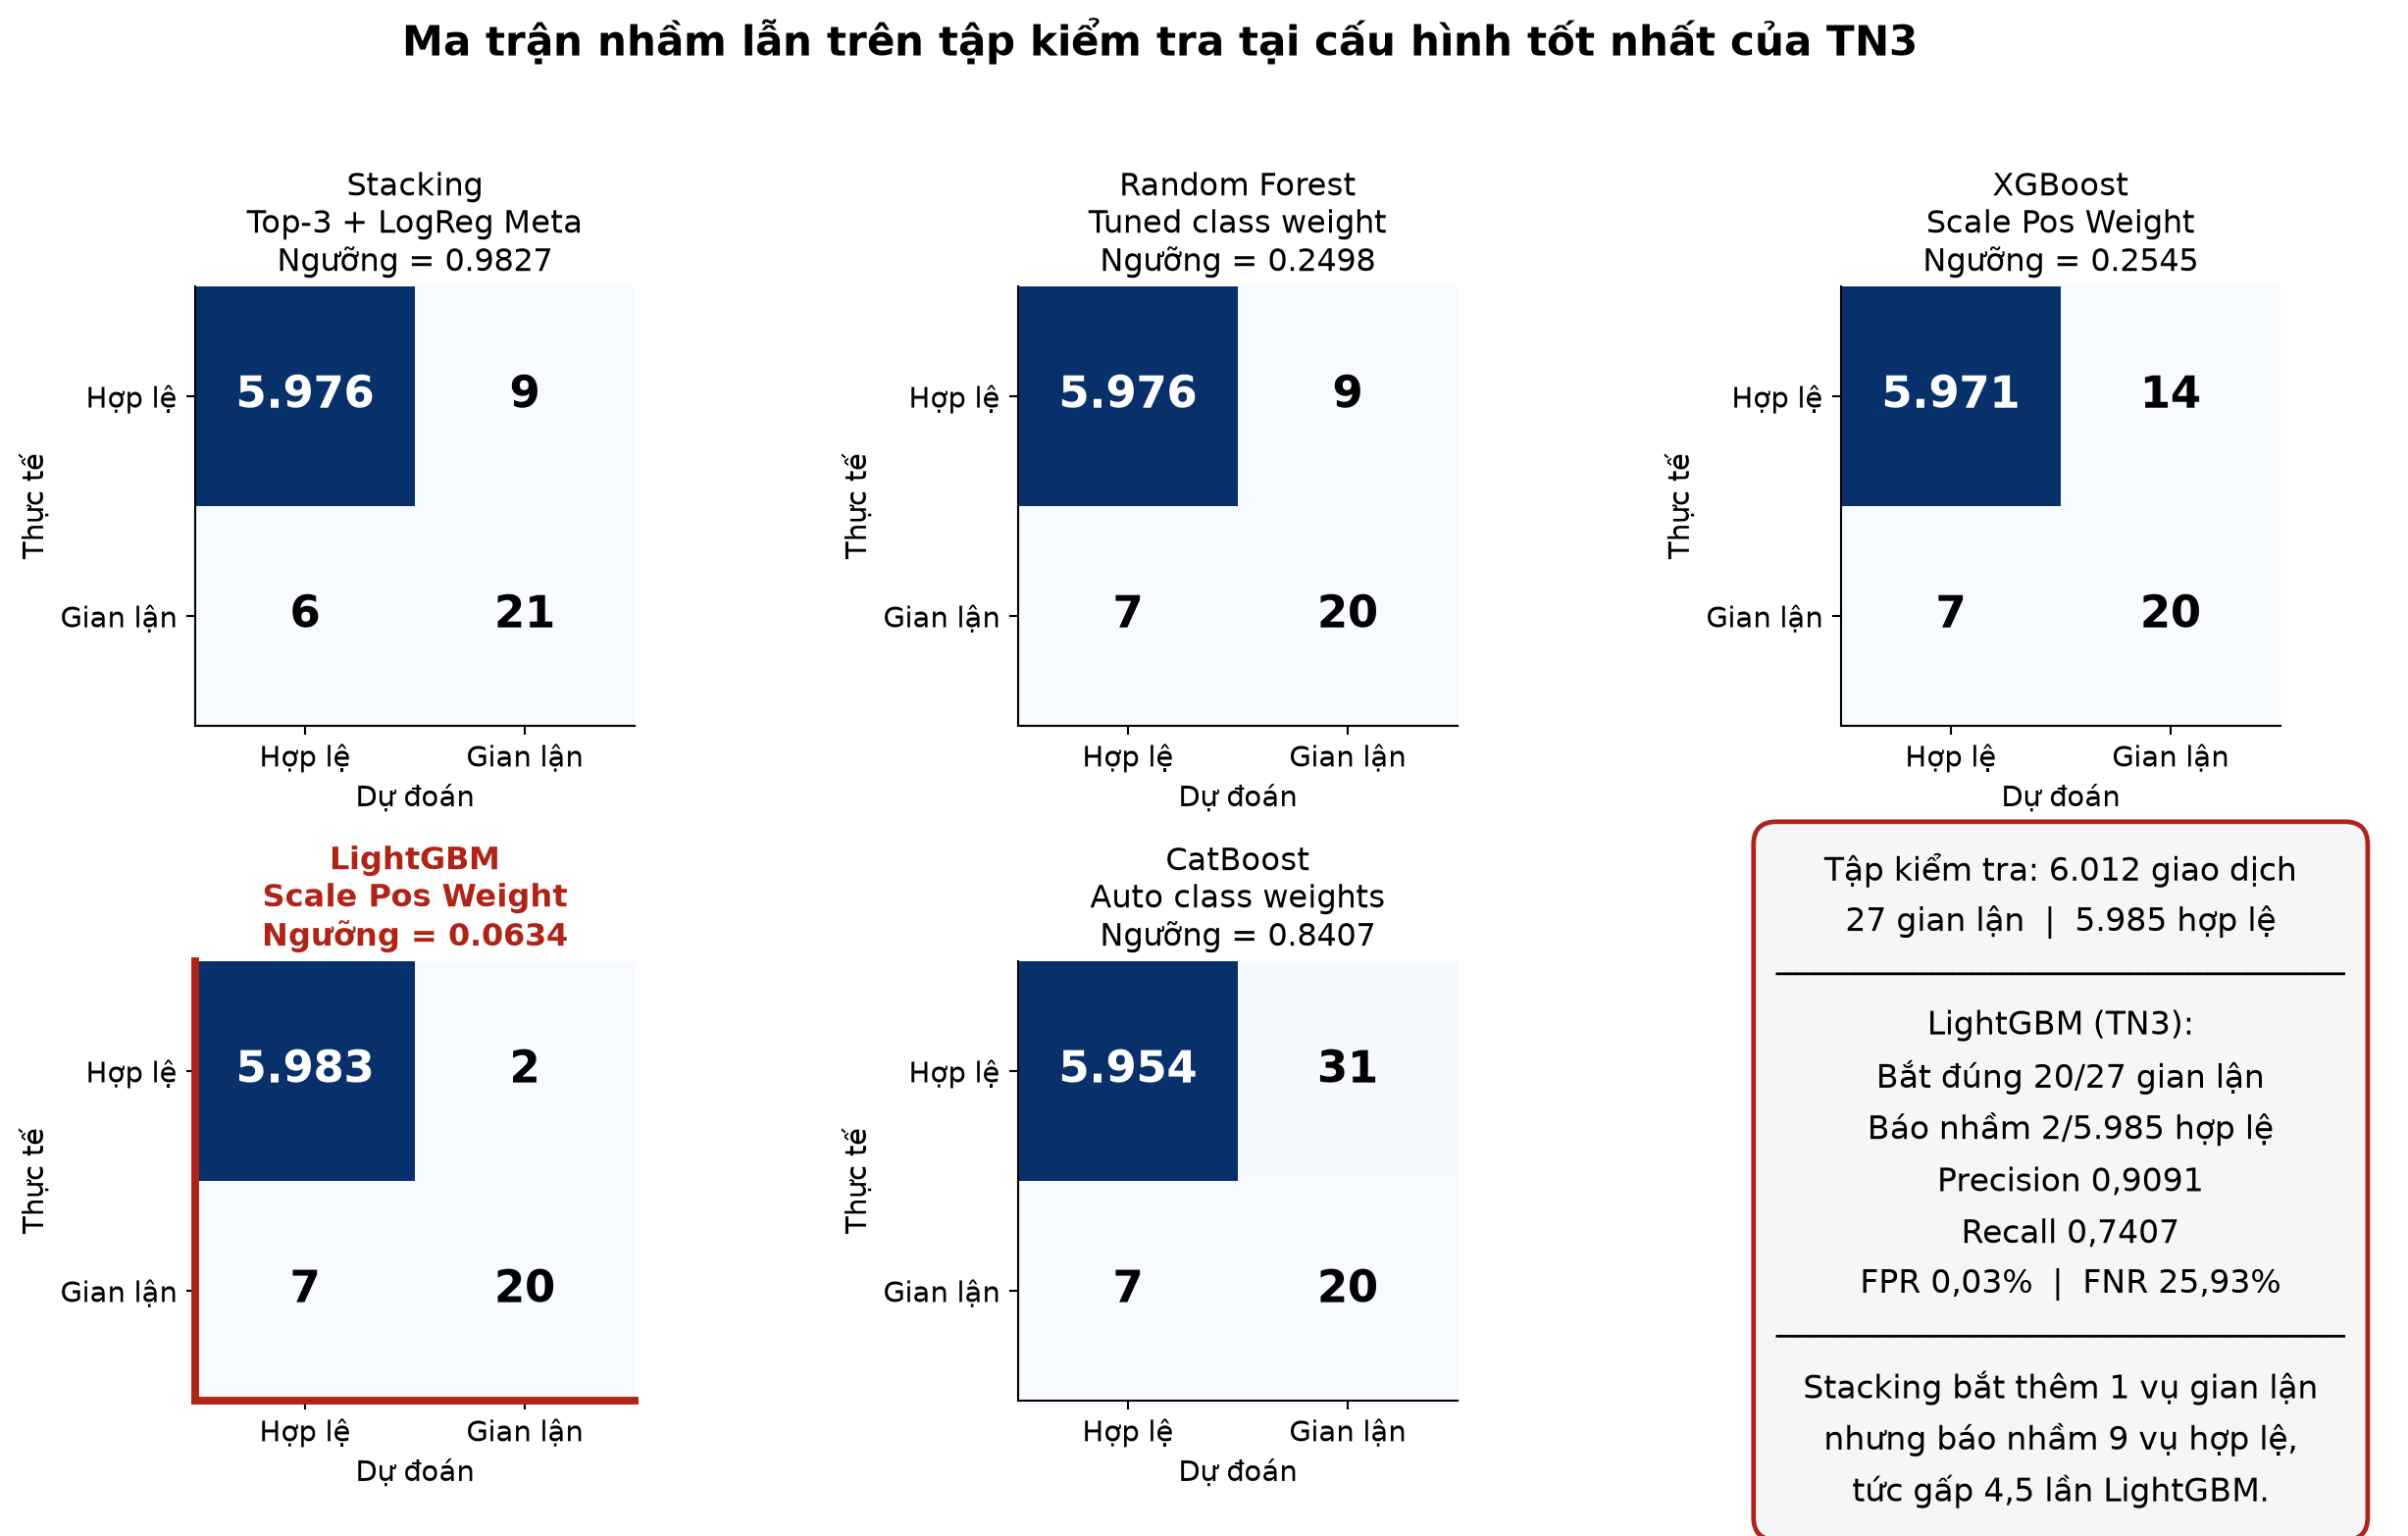
\includegraphics[width=\linewidth]{figures/fig_confusion_matrix.png}
    \caption{Ma trận nhầm lẫn của các mô hình tại cấu hình tốt nhất của thử nghiệm3 trên tập kiểm tra}
    \label{fig:confusion_matrix}
\end{figure}

Hình \ref{fig:confusion_matrix} trình bày ma trận nhầm lẫn của năm mô hình tại cấu hình tốt nhất của thử nghiệm3 trên tập kiểm tra. LightGBM phát hiện đúng 20 trong 27 giao dịch gian lận, bỏ sót 7, đồng thời chỉ báo nhầm 2 giao dịch hợp lệ --- con số thấp nhất trong năm mô hình. Stacking bắt được 21 trong 27 vụ, nhiều hơn đúng 1 vụ, nhưng phải chấp nhận 9 giao dịch hợp lệ bị báo nhầm, tức gấp 4{.}5 lần so với LightGBM; xét cả hai loại rủi ro thì Stacking không tốt bằng LightGBM. Ba mô hình còn lại cùng bắt 20 vụ nhưng báo nhầm lần lượt 9, 14 và 31 giao dịch hợp lệ. Xét theo tỷ lệ, FPR của LightGBM là 0{.}03\% trên 5\,985 giao dịch hợp lệ, tức thấp hơn tỷ lệ gian lận quan sát được là 0{.}45\%.

\begin{figure}[H]
    \centering
    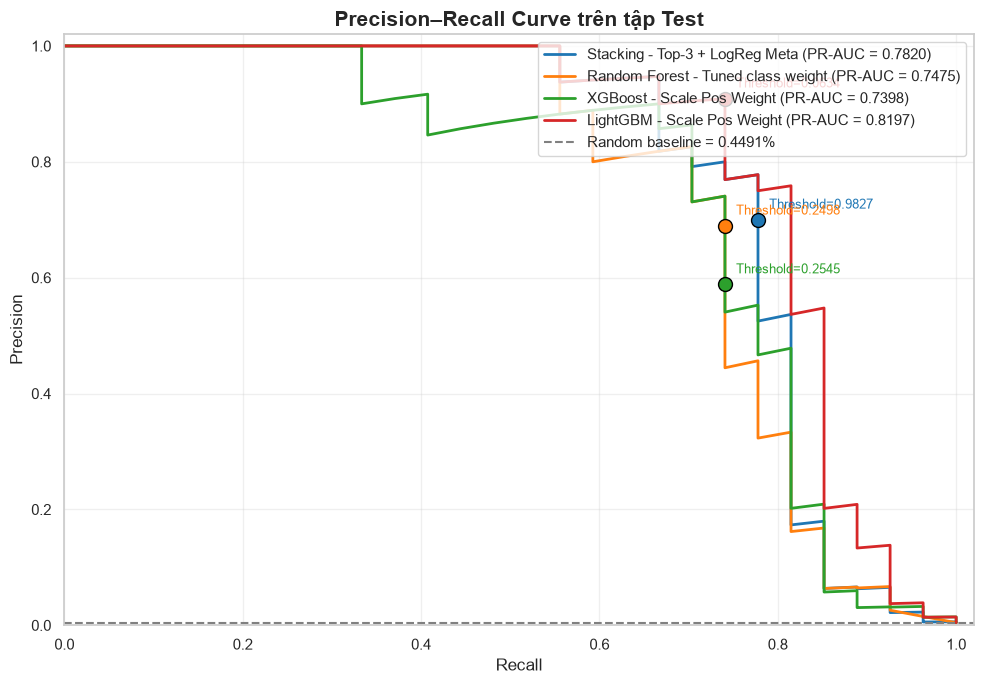
\includegraphics[width=0.9\linewidth]{figures/fig_pr_curve.png}
    \caption{Đường Precision--Recall của các mô hình tại cấu hình tốt nhất của thử nghiệm3 trên tập kiểm tra}
    \label{fig:pr_curve}
\end{figure}


\begin{figure}[H]
	\centering
	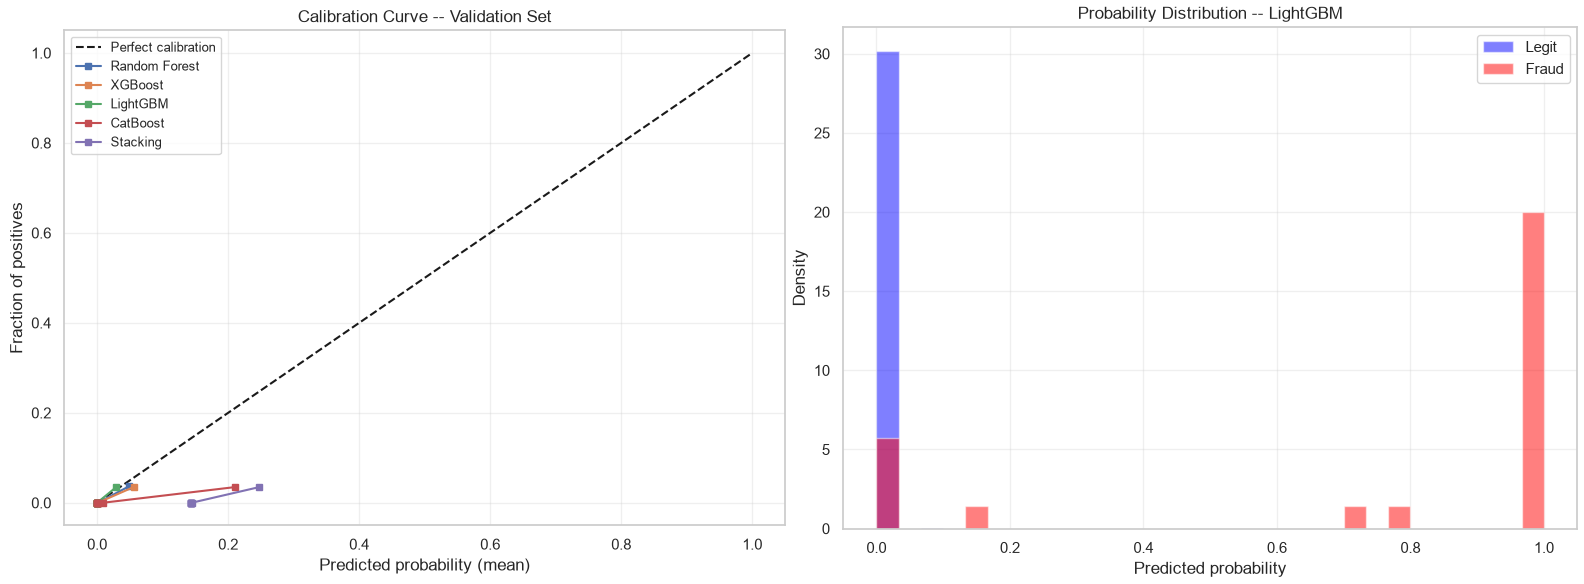
\includegraphics[width=\linewidth]{figures/fig_calibration_lightgbm.png}
	\caption{Đường hiệu chuẩn trên tập Validation và phân phối xác suất của mô hình LightGBM}
	\label{fig:calibration}
\end{figure}

Hình \ref{fig:pr_curve} vẽ đường Precision--Recall của bốn mô hình trên tập kiểm tra. Đường của LightGBM nằm cao hơn các đường còn lại trên hầu hết lân vùng thao tác thực tế, đạt PR-AUC 0{.}8197, tiếp theo là Stacking 0{.}7820, Random Forest 0{.}7475 và XGBoost 0{.}7398. Điểm hoạt động của LightGBM tại ngưỡng 0{.}0634 nằm ở vùng Recall cao với Precision 0{.}9091, tức độ chính xác cao gấp khoảng 202 lần so với dự đoán ngẫu nhiên. Đường nét đứt ngang là đường cơ sở ứng với tỷ lệ gian lận trong tập kiểm tra là 0{.}4491\%; toàn bộ các mô hình nằm trên đường này ở vùng ngưỡng đã chọn, xác nhận mô hình có giá trị thực tế.


Hình \ref{fig:calibration} bổ sung hai góc nhìn về chất lượng xác suất dự đoán. Đường hiệu chuẩn trên tập Validation cho thấy xác suất dự đoán của các mô hình thấp hơn đáng kể so với tần suất thực tế, một hạn chế chung của mô hình trên dữ liệu cực mất cân bằng. Biểu đồ phân phối xác suất của mô hình LightGBM cho thấy hai lớp tách biệt khá rõ: gần như toàn bộ giao dịch hợp lệ (99{.}94\%) tập trung ở vùng xác suất dưới 0{.}1, còn giao dịch gian lận tập trung ở vùng trên 0{.}8, với trung vị 0{.}997.

\section{Lựa chọn mô hình phù hợp với bộ dữ liệu}
Dựa trên sáu thử nghiệm, đề tài chọn LightGBM với \texttt{scale\_pos\_weight} trên tập 14 đặc trưng của thử nghiệm3 làm mô hình đề xuất cuối cùng. Lý do chọn được tóm tắt như sau:

\begin{itemize}
    \item Cân bằng tốt nhất trên ba chỉ số chính. LightGBM tại thử nghiệm3 đồng thời đạt F1-Score cao nhất (0{.}8163) và F2-Score cao nhất (0{.}7692) trong toàn bộ sáu thử nghiệm, với PR-AUC 0{.}8197 thuộc nhóm cao nhất. Như Bảng \ref{tab:exp_summary} cho thấy, không mô hình nào khác đạt đồng thời hai chỉ số F1 và F2 ở mức cao.
    \item Chi phí nghiệp vụ thấp nhất. Với Precision 0{.}9091, trong 22 giao dịch được cảnh báo có 20 là gian lận thật, tức chỉ 2 giao dịch hợp lệ bị kiểm tra lại không cần thiết --- tương đương FPR 0{.}0003. Đây là mức thấp nhất trong năm mô hình tại thử nghiệm3 và thấp hơn Stacking tới 5 lần (0{.}0015). Trong hệ thống thực tế, mỗi giao dịch hợp lệ bị chặn nhầm đều sinh chi phí xác minh và khiếu nại, nên đây là ưu thế quan trọng.
    \item Chi phí tính toán thấp. Thời gian dự đoán toàn bộ 6\,012 giao dịch là 0{.}0361 giây, nhanh nhất trong sáu thử nghiệm và thấp hơn thử nghiệm4 tới 2{.}9 lần; thời gian tinh chỉnh siêu tham số là 231{.}85 giây, giảm 4{.}9 lần so với thử nghiệm2 và 9{.}6 lần so với thử nghiệm4.
    \item Không đánh đổi nhiều Recall để lấy PR-AUC. thử nghiệm4 có PR-AUC cao hơn 0{.}0034 nhưng F2-Score thấp hơn 0{.}0058, FPR cao hơn và thời gian dự đoán gấp 2{.}9 lần. Với chỉ 27 mẫu gian lận trong tập kiểm tra, chênh lệch 0{.}0034 tương đương dưới 0{.}1\% và nằm trong biên sai số, không đủ căn cứ để đánh đổi.
\end{itemize}

Về hướng cải thiện Recall, vì bản chất nghiệp vụ ưu tiên bắt gian lận hơn là giảm báo nhầm, nếu hệ thống cần Recall cao hơn thì nên hạ ngưỡng quyết định của LightGBM xuống dưới 0{.}0634 thay vì đổi sang mô hình khác: theo đường Precision--Recall tại Hình \ref{fig:pr_curve}, hạ ngưỡng làm Recall tăng nhanh hơn đáng kể so với đổi mô hình, trong khi Precision giảm chậm. Ngưỡng vận hành cụ thể nên được chọn theo chi phí tương đối giữa một vụ gian lận bị bỏ sót và một giao dịch hợp lệ bị chặn nhầm, thay vì cố định theo F2-Score.

\section{Đánh giá tính khả thi và hạn chế}
\subsection{Điểm mạnh}
\begin{itemize}
    \item Quy trình hoàn chỉnh từ nạp dữ liệu, làm sạch, tạo đặc trưng đến huấn luyện và đánh giá, sát với bài toán phân loại nhị phân mất cân bằng trong thực tế.
    \item Thiết kế sáu thử nghiệm có kiểm soát: ba thử nghiệm tách ảnh hưởng của phương pháp mã hóa, ba thử nghiệm còn lại kiểm tra ảnh hưởng của việc loại bỏ đặc trưng, nhờ đó kết luận về tầm quan trọng của kỹ thuật tạo đặc trưng và của \texttt{TargetEncoder} có cơ sở thực nghiệm thay vì chỉ dựa trên kinh nghiệm.
    \item Khảo sát đồng thời bốn họ thuật toán rừng ngẫu nhiên và gradient boosting (XGBoost, LightGBM, CatBoost) cùng bốn chiến lược xử lý mất cân bằng khác nhau, đồng thời kết hợp các mô hình tốt nhất bằng stacking, bảo đảm khách quan khi so sánh hiệu quả.
    \item Thiết kế quy trình đánh giá nghiêm ngặt: tách riêng tập Fit, Validation và tập kiểm tra; giới hạn giá trị bất thường và chuẩn hóa chỉ học từ tập huấn luyện, giúp tránh rò rỉ dữ liệu.
    \item Sử dụng bộ chỉ số phù hợp với dữ liệu mất cân bằng gồm F2-Score và PR-AUC thay vì Accuracy, kèm báo cáo riêng FNR và FPR để phản ánh trực tiếp hai loại rủi ro của hệ thống.
\end{itemize}

\subsection{Hạn chế}
\begin{itemize}
    \item Bộ dữ liệu là dữ liệu mô phỏng với thời gian quan sát ngắn 10 ngày, chưa phản ánh đầy đủ các phương thức gian lận mới phát sinh theo thời gian.
    \item Tập kiểm tra chỉ chứa 27 giao dịch gian lận, nên mỗi giao dịch đúng thay đổi Recall khoảng 0{.}037. Chênh lệch PR-AUC giữa thử nghiệm3 và thử nghiệm4 là 0{.}0034, nhỏ hơn nhiều lần sai số này, khiến việc phân định thứ hạng giữa hai cấu hình chưa thật sự chắc chắn.
    \item Đặc trưng khoảng cách \texttt{distance\_km} tạo ra từ vị trí địa lý chứa nhiễu do chất lượng dữ liệu tọa độ, có thể làm giảm hiệu quả của mô hình.
    \item Xác suất dự đoán của các mô hình chưa được hiệu chuẩn tốt trên tập Validation, ảnh hưởng đến việc diễn giải ngưỡng quyết định theo xác suất tuyệt đối.
    \item Các khoảng siêu tham số được khảo sát bằng tìm kiếm ngẫu nhiên với số lần thử có giới hạn, chưa khẳng định được cấu hình tối ưu toàn cục.
\end{itemize}

\section{Hướng phát triển trong tương lai}
\begin{itemize}
    \item Mở rộng dữ liệu thực tế nhiều tháng và bổ sung các đặc trưng như dấu vân tay thiết bị, địa chỉ IP, lịch sử tranh chấp của thẻ.
    \item Thử thêm các tổ hợp loại bỏ đặc trưng khác, so sánh \texttt{TargetEncoder} với \texttt{CatBoostEncoder} và mã hóa theo chuỗi thời gian, nhằm cải thiện thêm Recall.
    \item Hiệu chuẩn xác suất dự đoán bằng \texttt{CalibratedClassifierCV} và chọn ngưỡng vận hành theo chi phí kinh doanh thay vì chỉ theo F2-Score.
    \item Áp dụng các kỹ thuật nâng cao như điều chỉnh trọng số lớp theo chi phí nghiệp vụ, học sâu trên chuỗi giao dịch, hoặc tinh chỉnh siêu tham số có hệ thống bằng tối ưu hóa Bayes.
    \item Mở rộng stacking với nhiều mô hình cơ sở và bộ tổng hợp khác nhau.
    \item Triển khai hệ thống chấm điểm theo thời gian thực với giám sát độ trễ và phát hiện lệch phân bố dữ liệu sau khi đưa vào vận hành.
\end{itemize}
